\section{Selections}
\label{Selections}
\subsection{Global Event Selections}
Only events with less than 8000 VELO clusters are considered in this analysis, as imposed by the trigger requirements. When measuring \psitwos-to-\jpsi production ratio, the bias caused by this global cut is negligible since the data sample with more than 8000 VELO clusters account for less than $0.1\%$. All events are also required to have exactly one reconstructed primary vertex to avoid pile-up.
For the equivalence of VELO acceptance, we also need to restrict the z-coordinate of primary vertex. The restriction is made according to which multiplicity variable we choose to represent the charged particle multiplicity. As an example, Figure~\ref{JpsiPVZ} shows the $N_{\rm tracks}^{\rm PV}$ distribution in different PVZ ranges. We remove the data within which the $N_{\rm tracks}^{\rm PV}$ distribution is clearly deviated, which is $z_{PV}<-30$ mm in this case. The PVZ restrictions for other cases is summarized in Table~\ref{TablePVZ}.
\begin{table}[H]
\caption{Global cuts on $z_{PV}$.}
\begin{center}
\begin{tabular}{lll}
\hline
\textbf{Configuration} & \textbf{Mult. Variable} & \textbf{$z_{PV}$}\\
\hline
	$p$Pb & $N_{\rm tracks}^{\rm PV}$ & [-30, 180] mm\\
	$p$Pb & $N_{\rm fwd}^{\rm PV}$ & [-180, 180] mm\\
	$p$Pb & $N_{\rm bwd}^{\rm PV}$ & [-30, 180] mm\\
	Pb$p$ & $N_{\rm tracks}^{\rm PV}$ & [-60, 180] mm\\
        Pb$p$ & $N_{\rm fwd}^{\rm PV}$ & [-180, 120] mm\\
        Pb$p$ & $N_{\rm bwd}^{\rm PV}$ & [-30, 180] mm\\
\hline
\end{tabular}
\end{center}
\label{TablePVZ}
\end{table}

\begin{figure}[!tbp]
\begin{center}
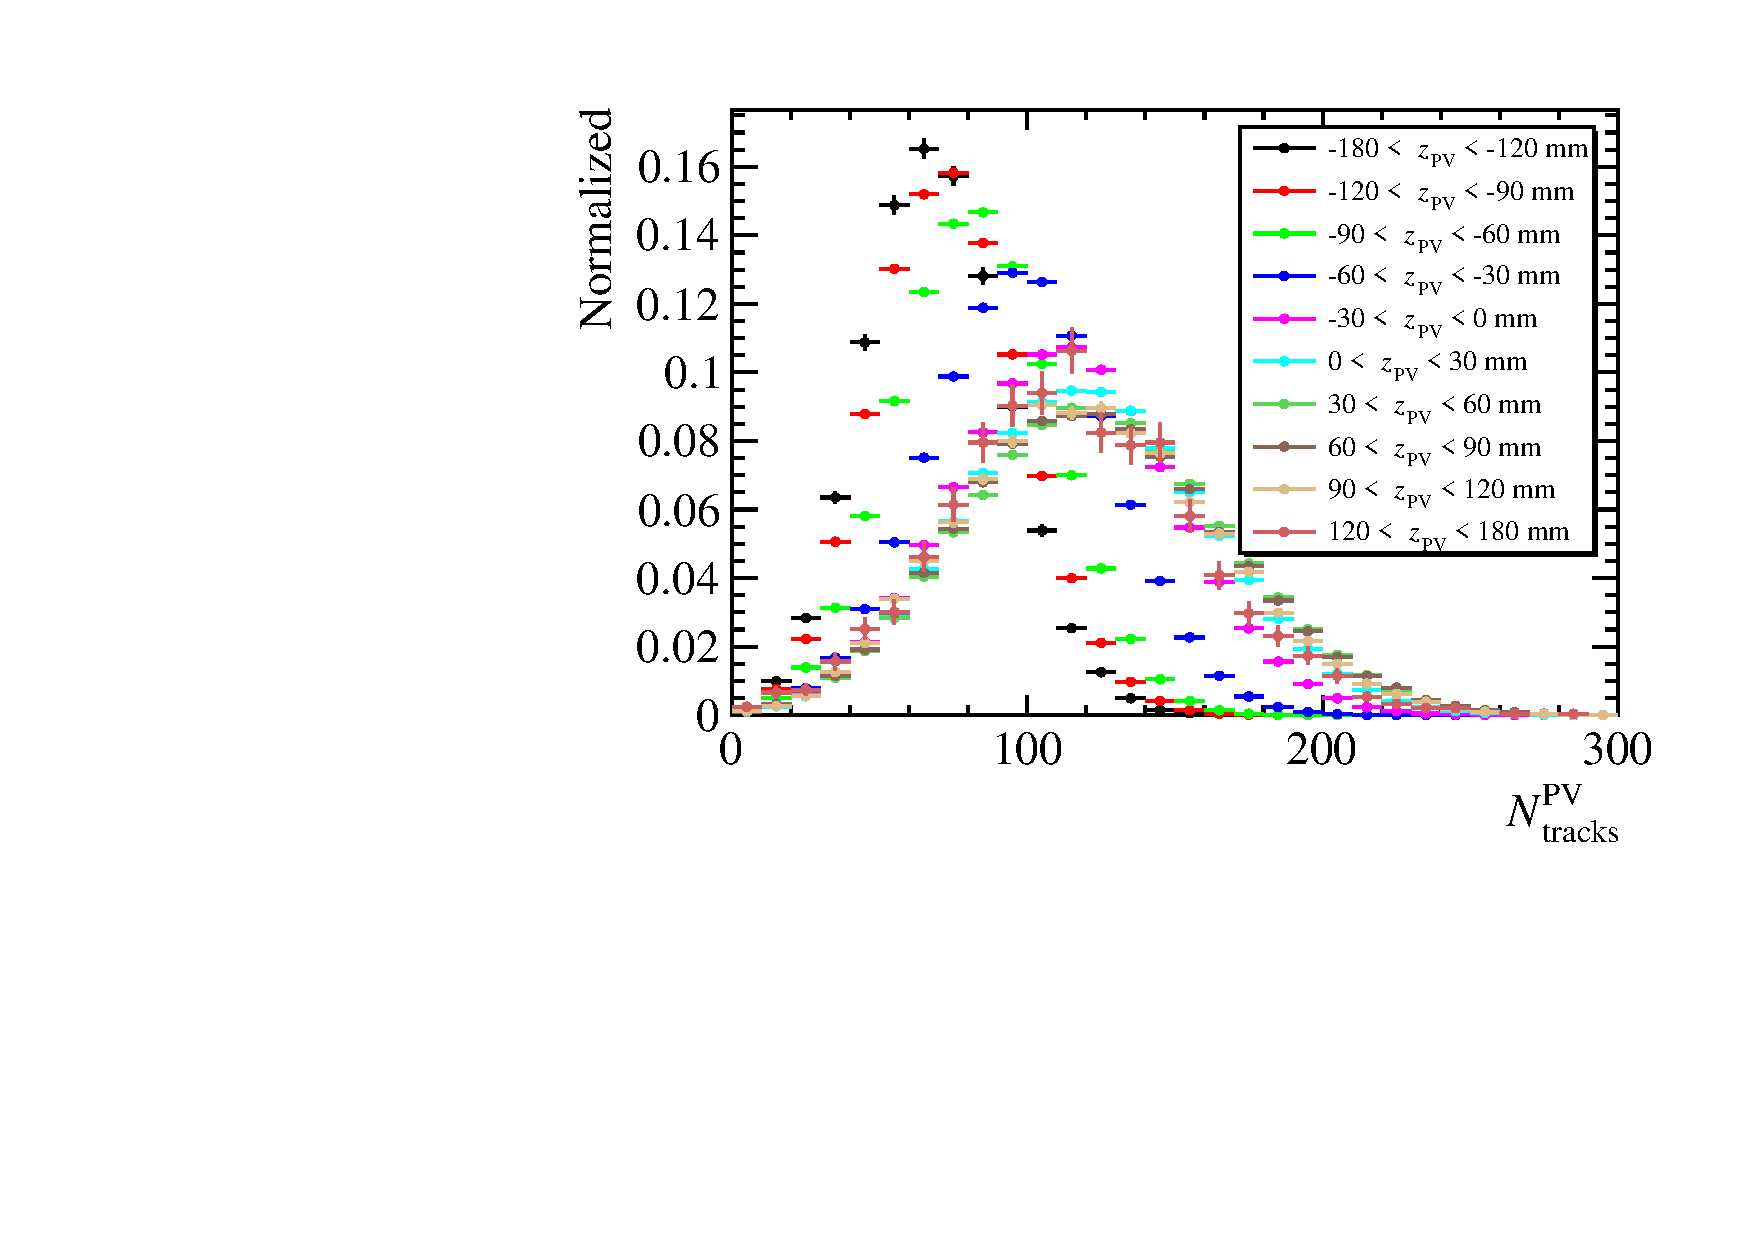
\includegraphics[width=0.7\linewidth]{pdf/pPb/Workdir/PVZvsMul/Jpsi.pdf}
\end{center}
\caption{
    Distribution of $N_{\rm tracks}^{\rm PV}$ in different $z_{PV}$ ranges for \jpsi in $p$Pb collisions.}
\label{JpsiPVZ}
\end{figure}

\subsection{Candidate Selection}
The \jpsi and \psitwos candidates are formed from two oppositely charged muons coming from a common vertex. Both decay modes are using same selection criteria. They are required to be TOS (Trigger On Signal) for the L0Muon and Hlt1DiMuonHighMas trigger lines, i.e. that the reconstructed candidate or its decay products are associated with a trigger object fulfilling the trigger requirements. Then the candidates used are directly the ones selected by the line Hlt2DiMuonJPsiTurbo and Hlt2DiMuonPsi2STurbo lines respectively, in the TURBO stream, without offline reconstruction. 
Additional cuts are applied at the analysis level. Muon tracks have to be in the geometrical acceptance of the spectrometer ($2 < \eta < 5$) and to have \pt $>$ 900 \mevc in order to improve the signal over background ratio. Both tracks are required to have a good fit quality, $\chi^2/ndof < 3$ and a ghost probability less than 0.4. They are identified as muons by requiring ProbNN($\mu$) $>$ 0.9 for both \jpsi and \psitwos. This is a harsh but appropriate PID cut since it can significantly reduce the background of high-multiplicity \psitwos data sample. And for low-multiplicity region, it doesn't remove too much of the signals. We can therefore achieve relative low statistical uncertainties when fitting the invariant mass spectrum and pseudo decay time spectrum, since the dominant uncertainties are statistical uncertainties of \psitwos which will be discuss later. The comparison for high- and low-multiplicity region of loose PID cut (ProbNN($\mu$) $>$ 0.6) and tight PID cut (ProbNN($\mu$) $>$ 0.9) can be seen in Figure~\ref{ProbNNmu}.
In addition, for both \jpsi and \psitwos, the two muons are required to form a good vertex asking the vertex fit probability Prob($\chi^2$) $>$ $0.5\%$. The \psitwos and \jpsi candidates are required to have a mass within 120 MeV/c2 of the PDG value. All selection criteria are specified in Table~\ref{OfflineSelection}.
\begin{table}[H]
\caption{Offline selection for \jpsi and \psitwos.}
\begin{center}
\begin{tabular}{ll}
\hline
\textbf{Variable} & \textbf{Cuts}\\
\hline
	$\mu^{\pm} \eta$ & $2<\eta<5$\\
	$\mu^{\pm} \pt$ & $>$900 \mevc\\
	ProbNNmu & $>$0.9\\
	TrackGhost Prob. & $<$0.4\\
	Vertex $\chi^2$ Prob. & $>0.5\%$\\
	Track $\chi^2/ndof$ & $<$3\\
	mass window & $\pm$ 120 \mevcc\\
\hline
\end{tabular}
\end{center}
\label{OfflineSelection}
\end{table}
\begin{figure}[!tbp]
\begin{center}
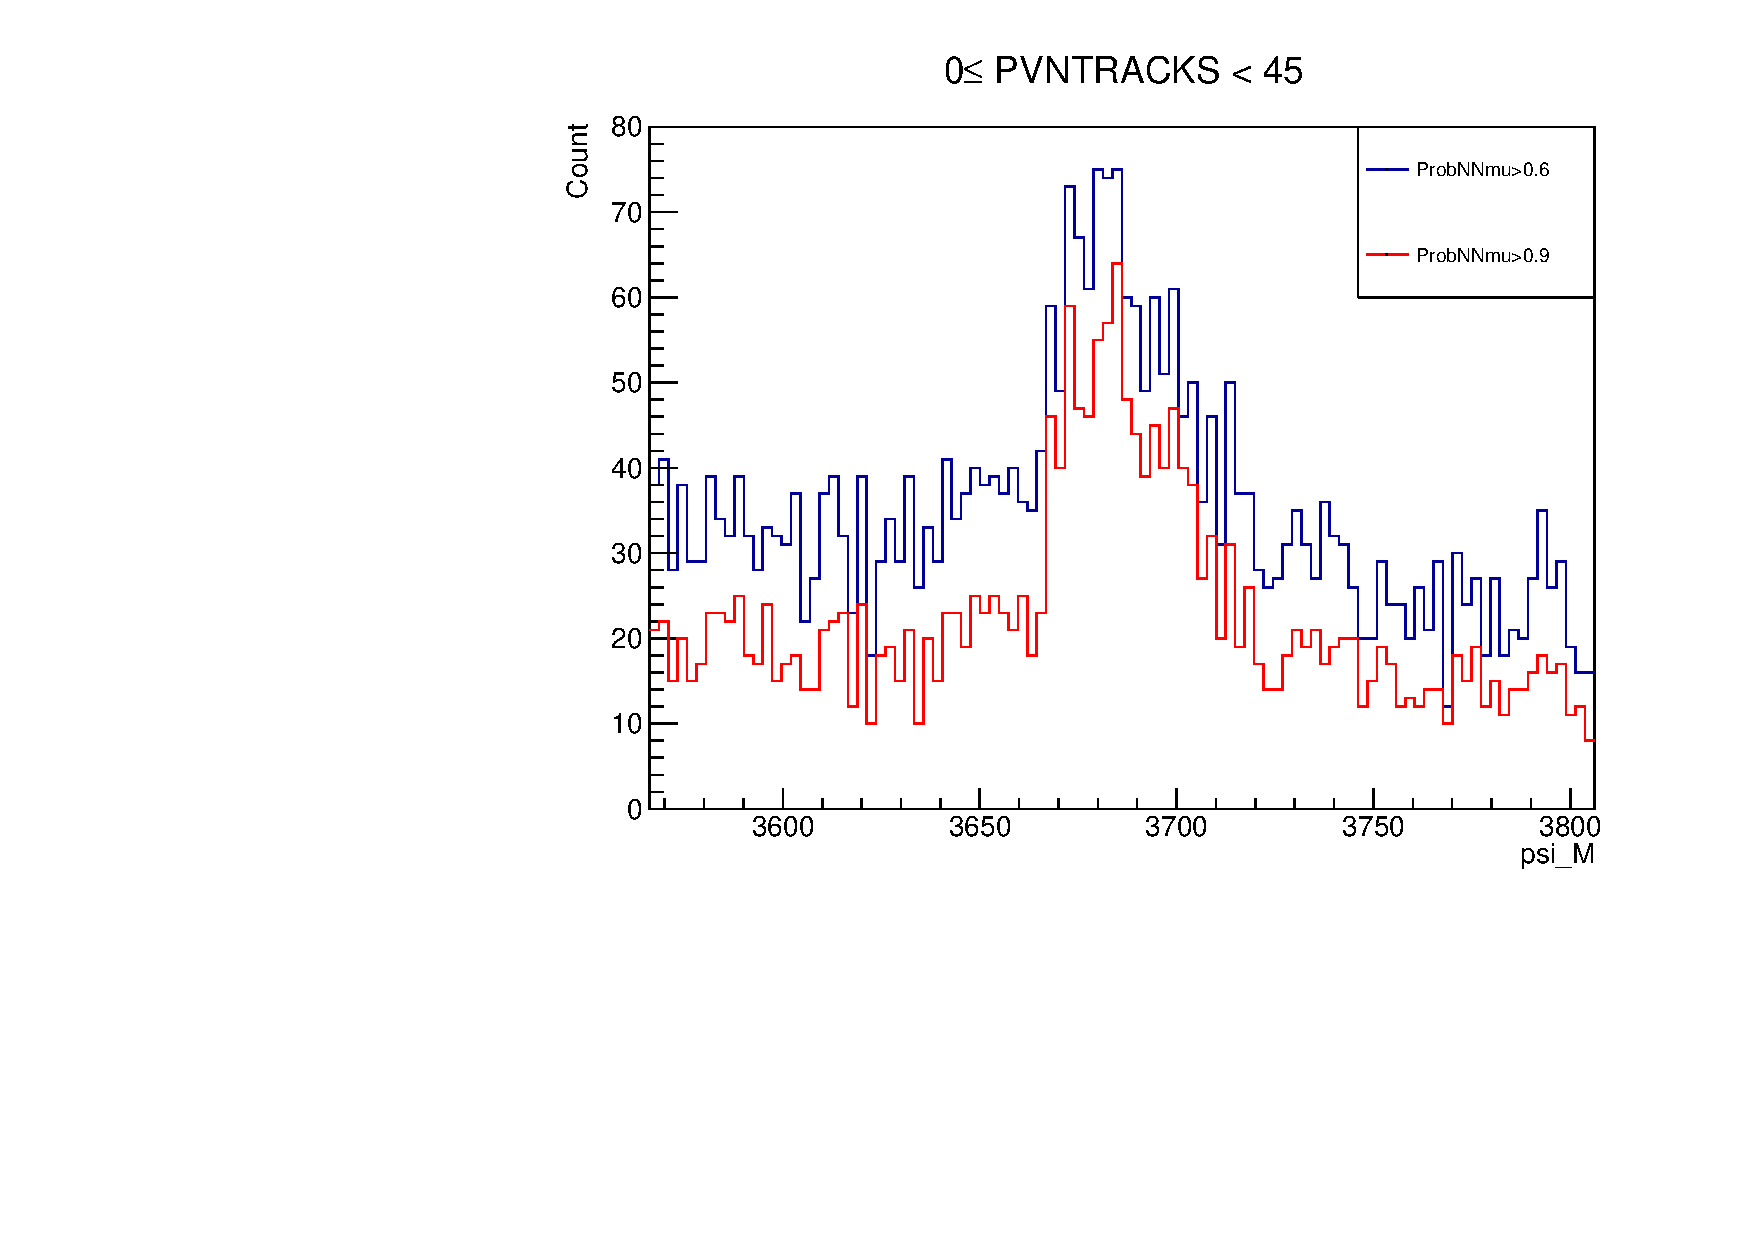
\includegraphics[width=0.7\linewidth]{pdf/pPb/Workdir/Psi_M_ProbNNmu/Low.pdf}
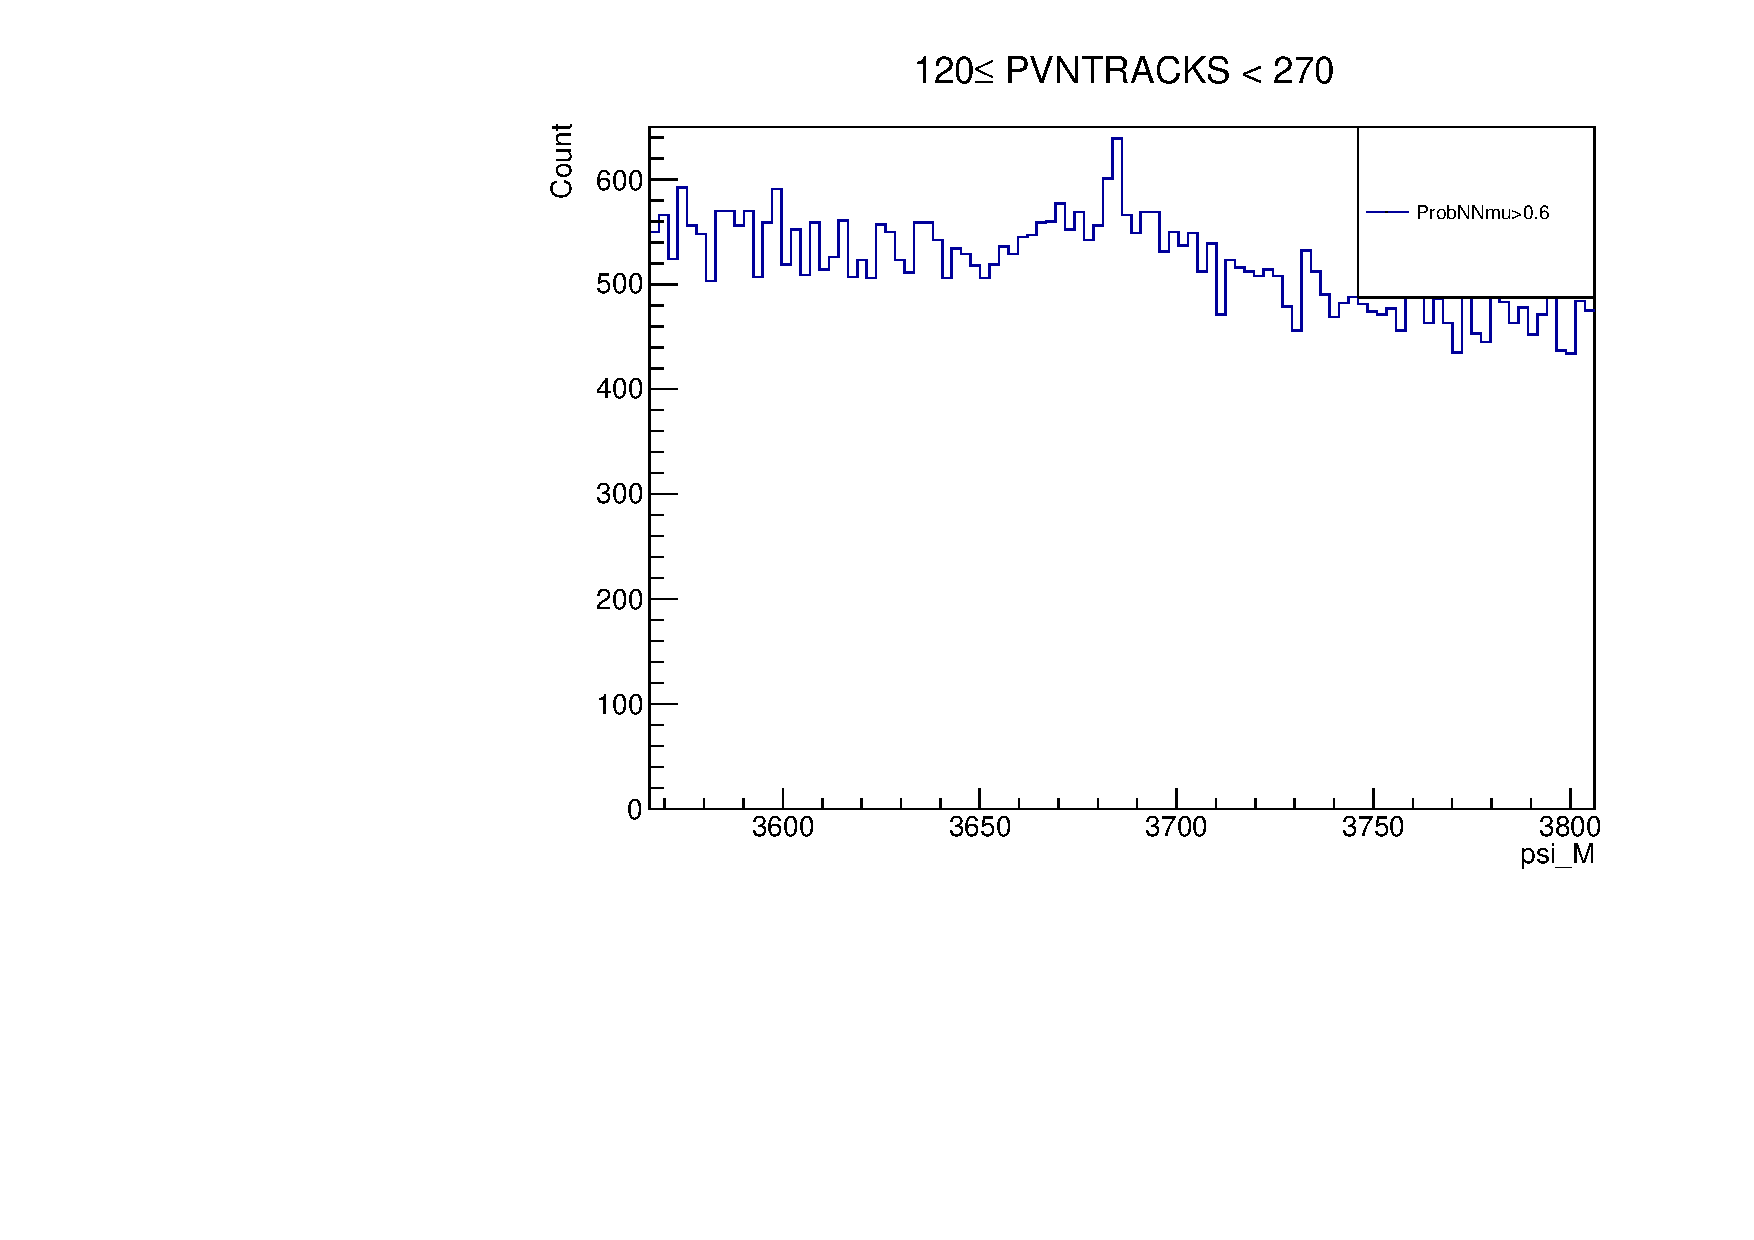
\includegraphics[width=0.49\linewidth]{pdf/pPb/Workdir/Psi_M_ProbNNmu/High1.pdf}
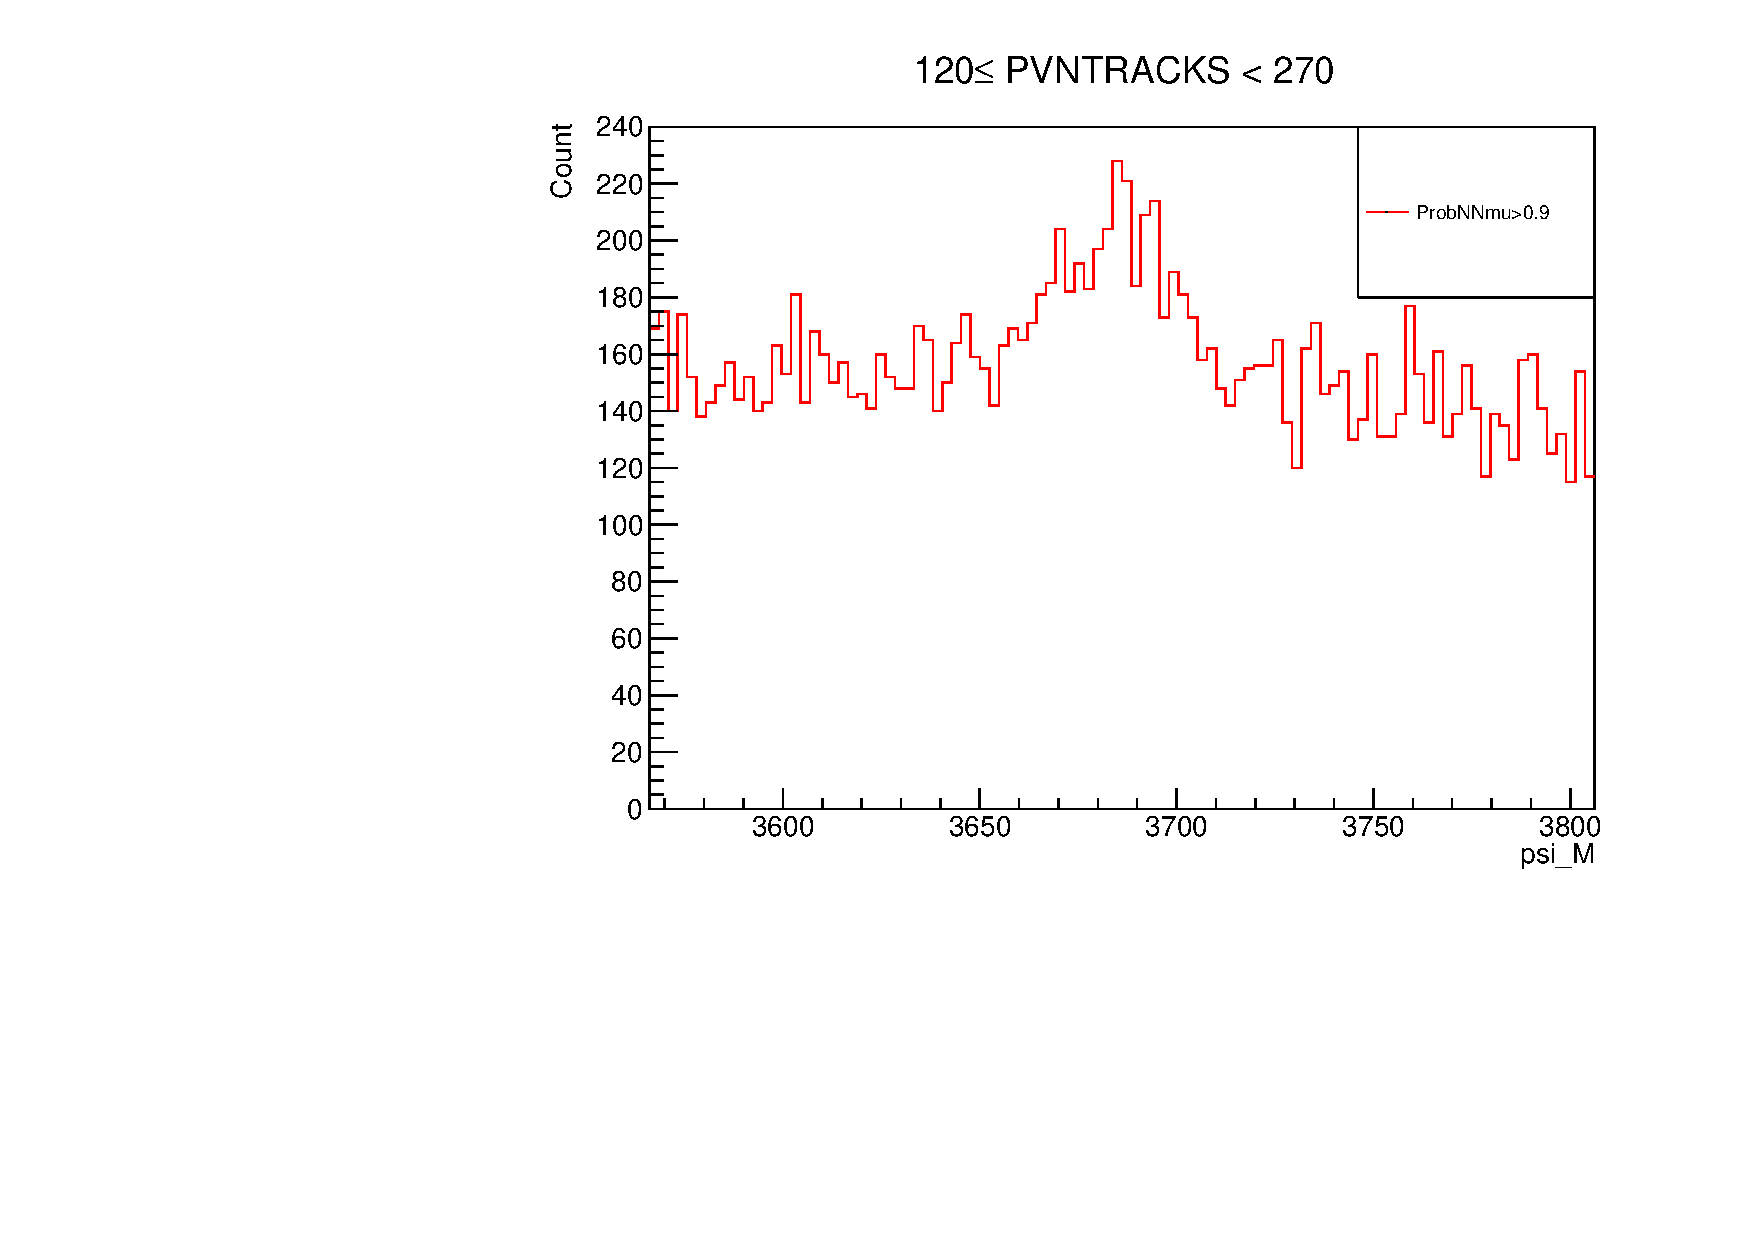
\includegraphics[width=0.49\linewidth]{pdf/pPb/Workdir/Psi_M_ProbNNmu/High2.pdf}
\end{center}
\caption{
	Mass spectrum of \psitwos after online and offline cuts with loose PID cut (blue) and tight PID cut (red). The first row is for lowest-multiplicity class and the second row is for highest-multiplicity class.}
\label{ProbNNmu}
\end{figure}

